The BHTs generated by BibleGoAI are served to end users through \textbf{BibleGo.org}, a web application built with Next.js \citep{nextjs}, React, and TypeScript, backed by a PostgreSQL database and hosted on Vercel. The platform reaches approximately 100--300 unique users per month, with monthly page-view volumes ranging from ${\sim}200$ to ${\sim}2{,}500$ depending on seasonal and community activity. This section briefly describes the served interface so that the BHTs evaluated in Section~\ref{sec:evaluation} can be situated in their delivered form; full deployment details are out of scope for this paper.

\paragraph{Reading interface.}
The main reading interface (Figure~\ref{fig:desktop-bht}) presents a two-column layout: the NASB Bible text with inline original-language tags on the left, and a commentary panel on the right. When a user selects a verse, the corresponding BHT is displayed along with footnotes that link each sentence to its source commentary; users can expand individual footnotes to view the original quotes, the commentator attribution, and a similarity score. Each commentator's full excerpt is also available as a separate card, enabling side-by-side comparison of perspectives. On mobile the commentary panel appears as a slide-up drawer (Figure~\ref{fig:bht-mobile}). A separate full-commentary mode is also available, in which readers can browse the complete chapter-level text from any individual commentator.

\begin{figure}[t]
  \centering
  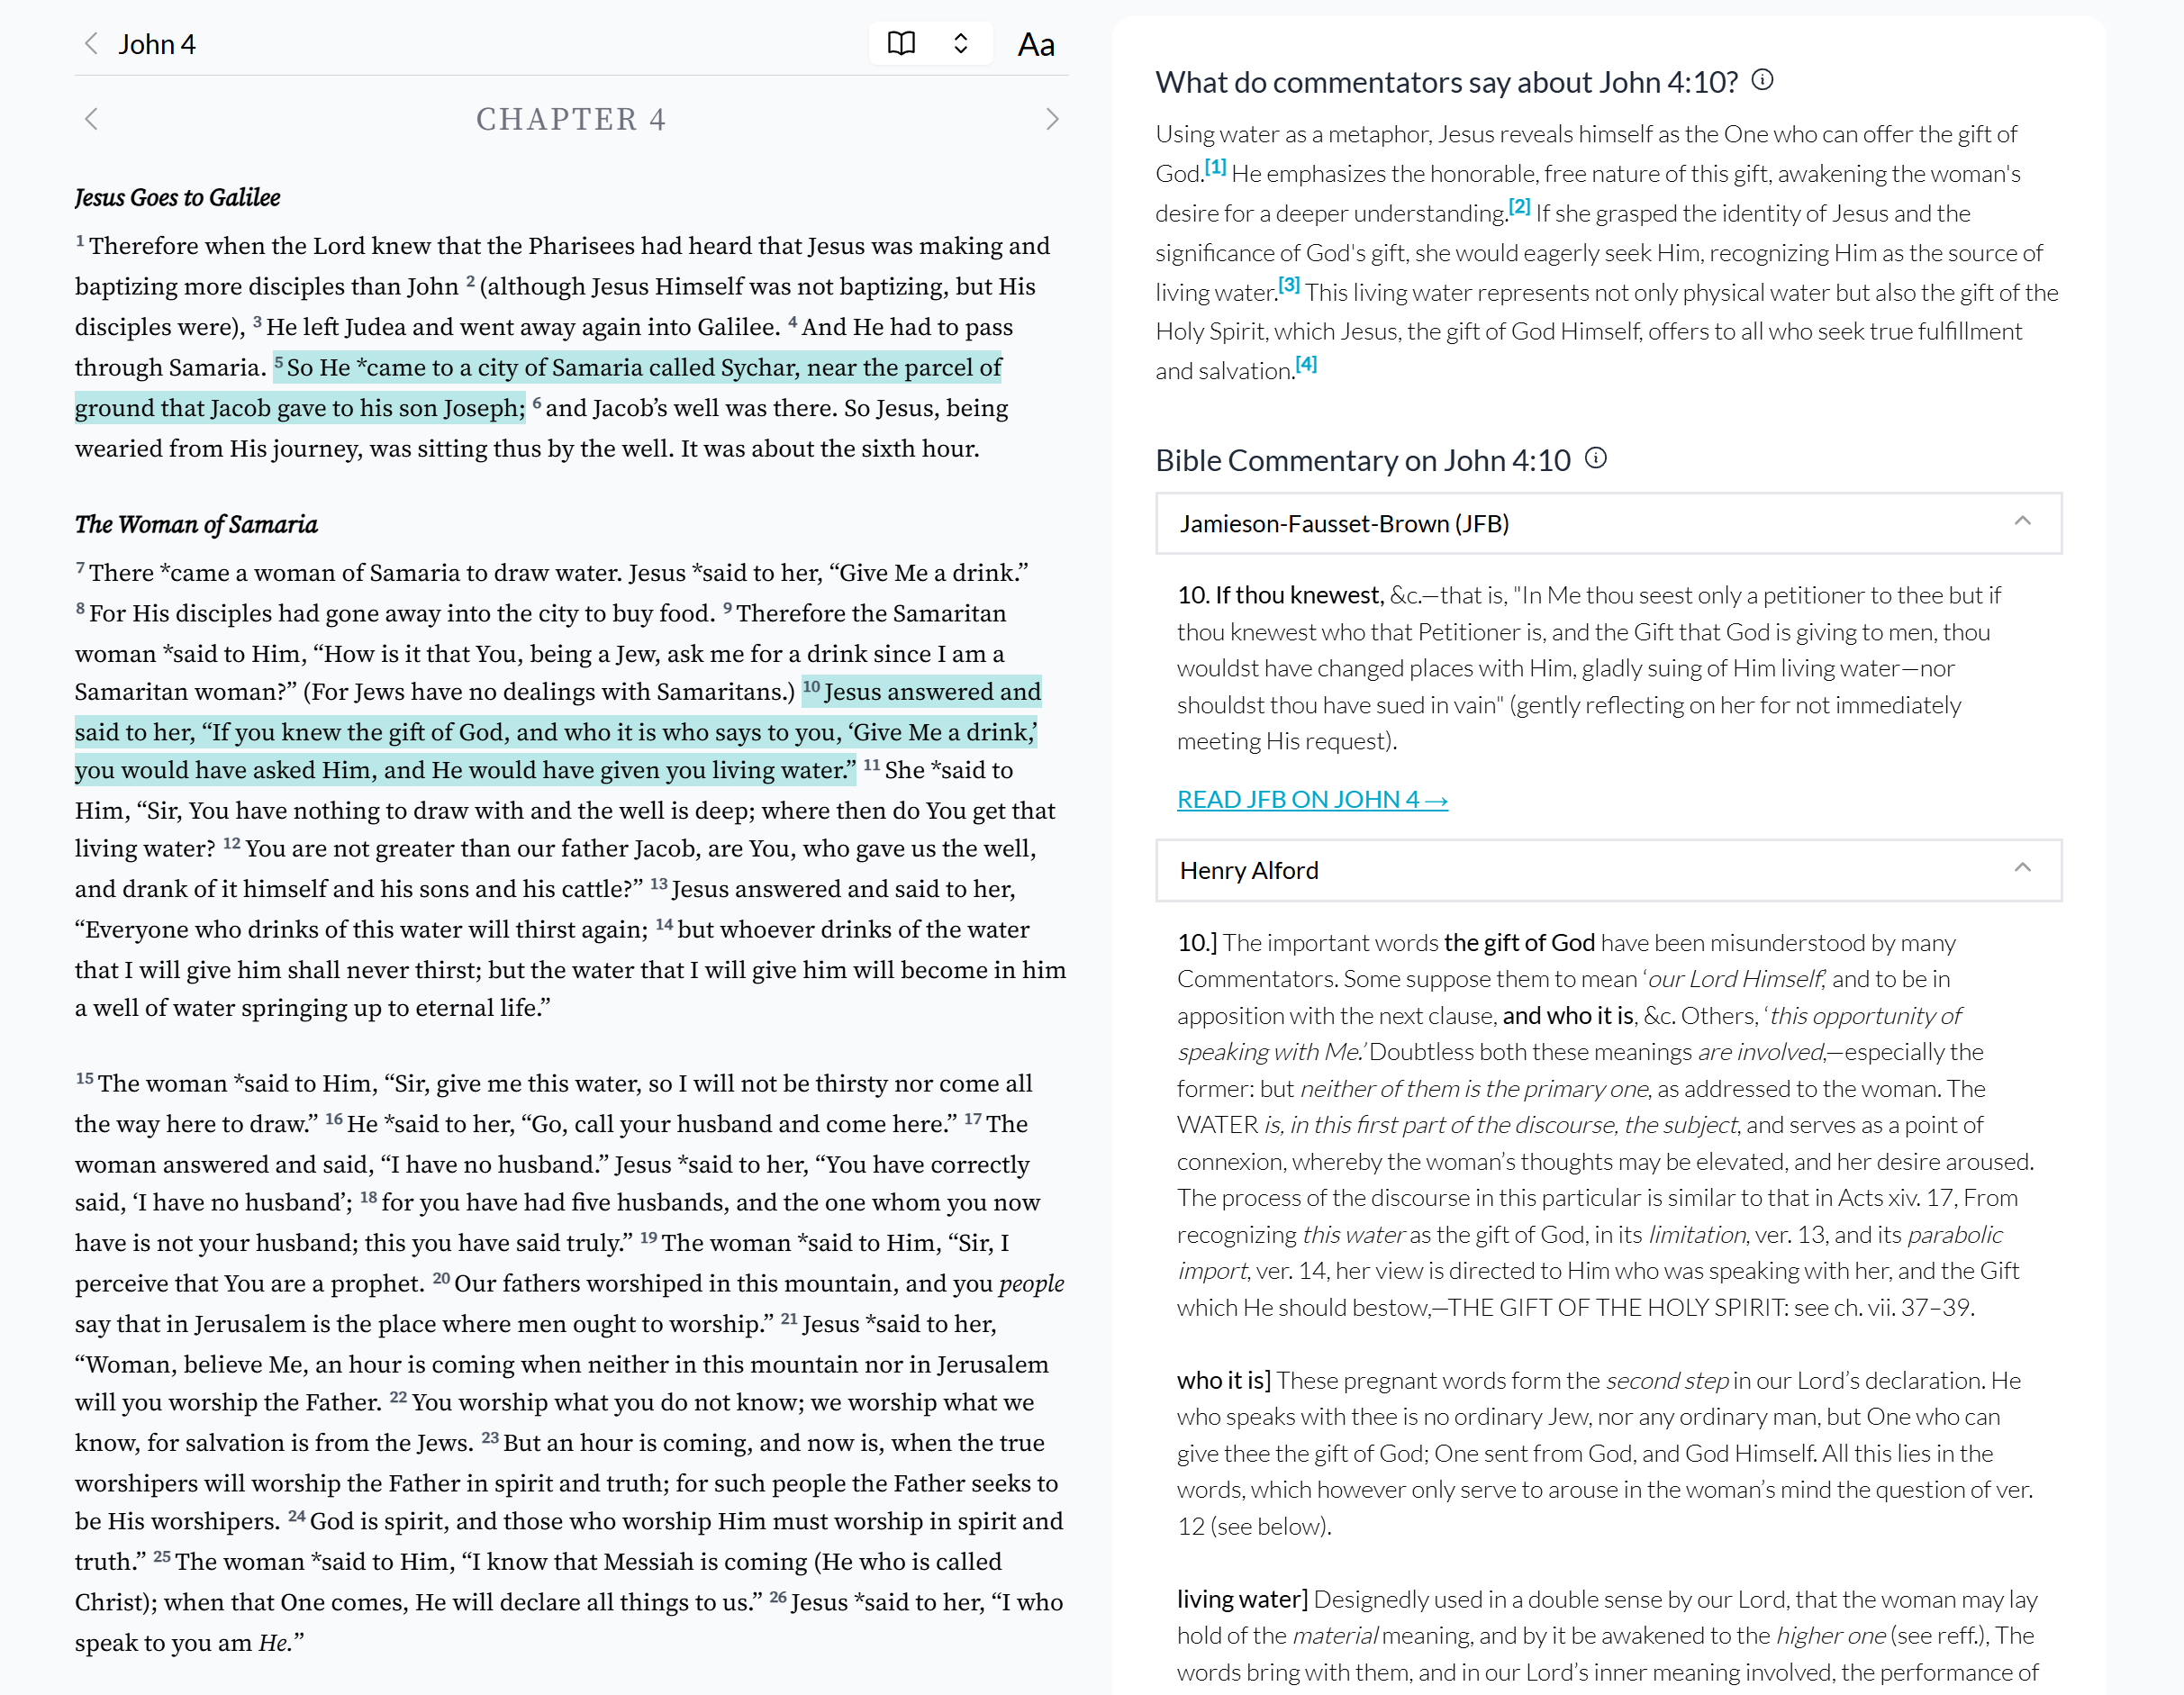
\includegraphics[width=\columnwidth]{figures/biblego-desktop-bht.png}
  \caption{The BibleGo.org desktop reading interface. The two-column layout presents the NASB Bible text with inline original-language tags (left) alongside the BHT commentary panel (right), in which footnotes link each sentence back to its source commentator.}
  \label{fig:desktop-bht}
\end{figure}

\begin{figure}[t]
  \centering
  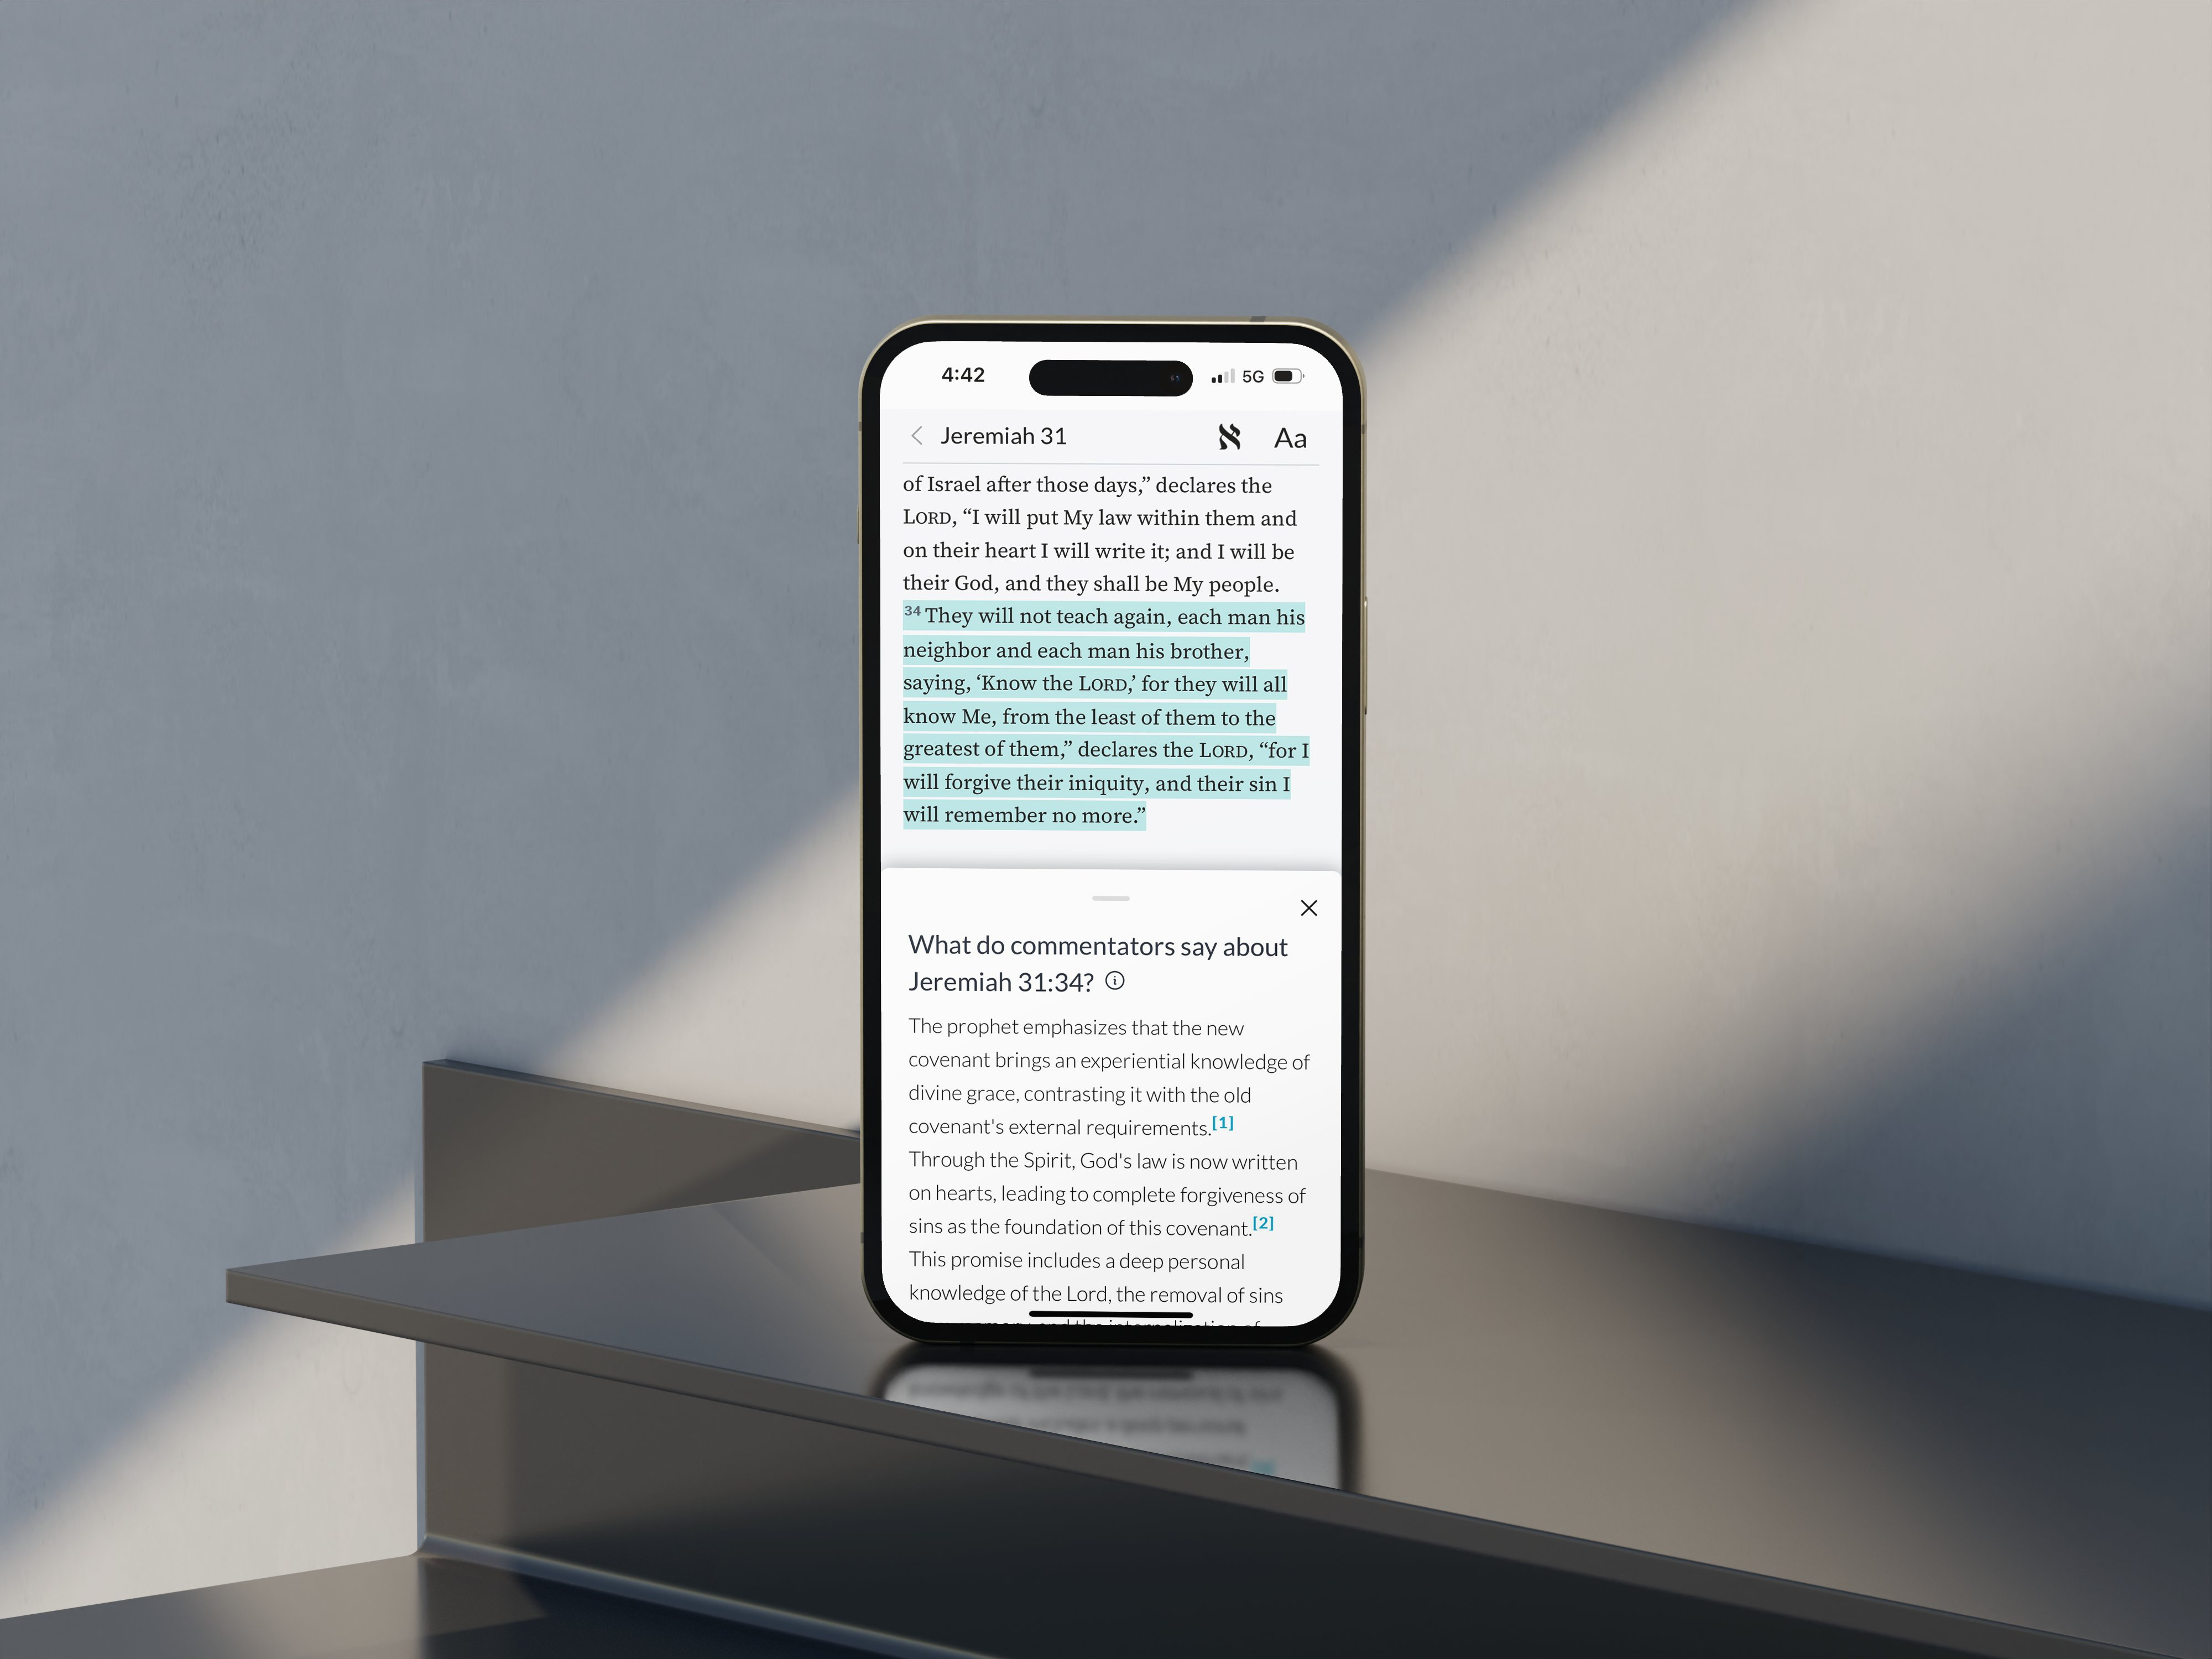
\includegraphics[width=0.75\columnwidth]{figures/biblego-bht-mobile.jpg}
  \caption{The BibleGo.org mobile experience with the BHT commentary drawer. Footnotes (numbered markers) link each sentence back to its source commentator, allowing users to trace every claim to the original commentary.}
  \label{fig:bht-mobile}
\end{figure}

\paragraph{Word study.}
BibleGo.org also includes an interactive word-study feature, the \textit{Word Donut}, powered by Strong's concordance data built from the original-language tagging pipeline (Section~\ref{sec:architecture}). A user can select any word in the Bible text to view its original Greek or Hebrew form, transliteration, and definition; an interactive doughnut chart then visualizes how the NASB translators rendered that word across all of its biblical occurrences (Figure~\ref{fig:word-donut}). The same widget is available on mobile via the reading drawer.

\begin{figure}[t]
  \centering
  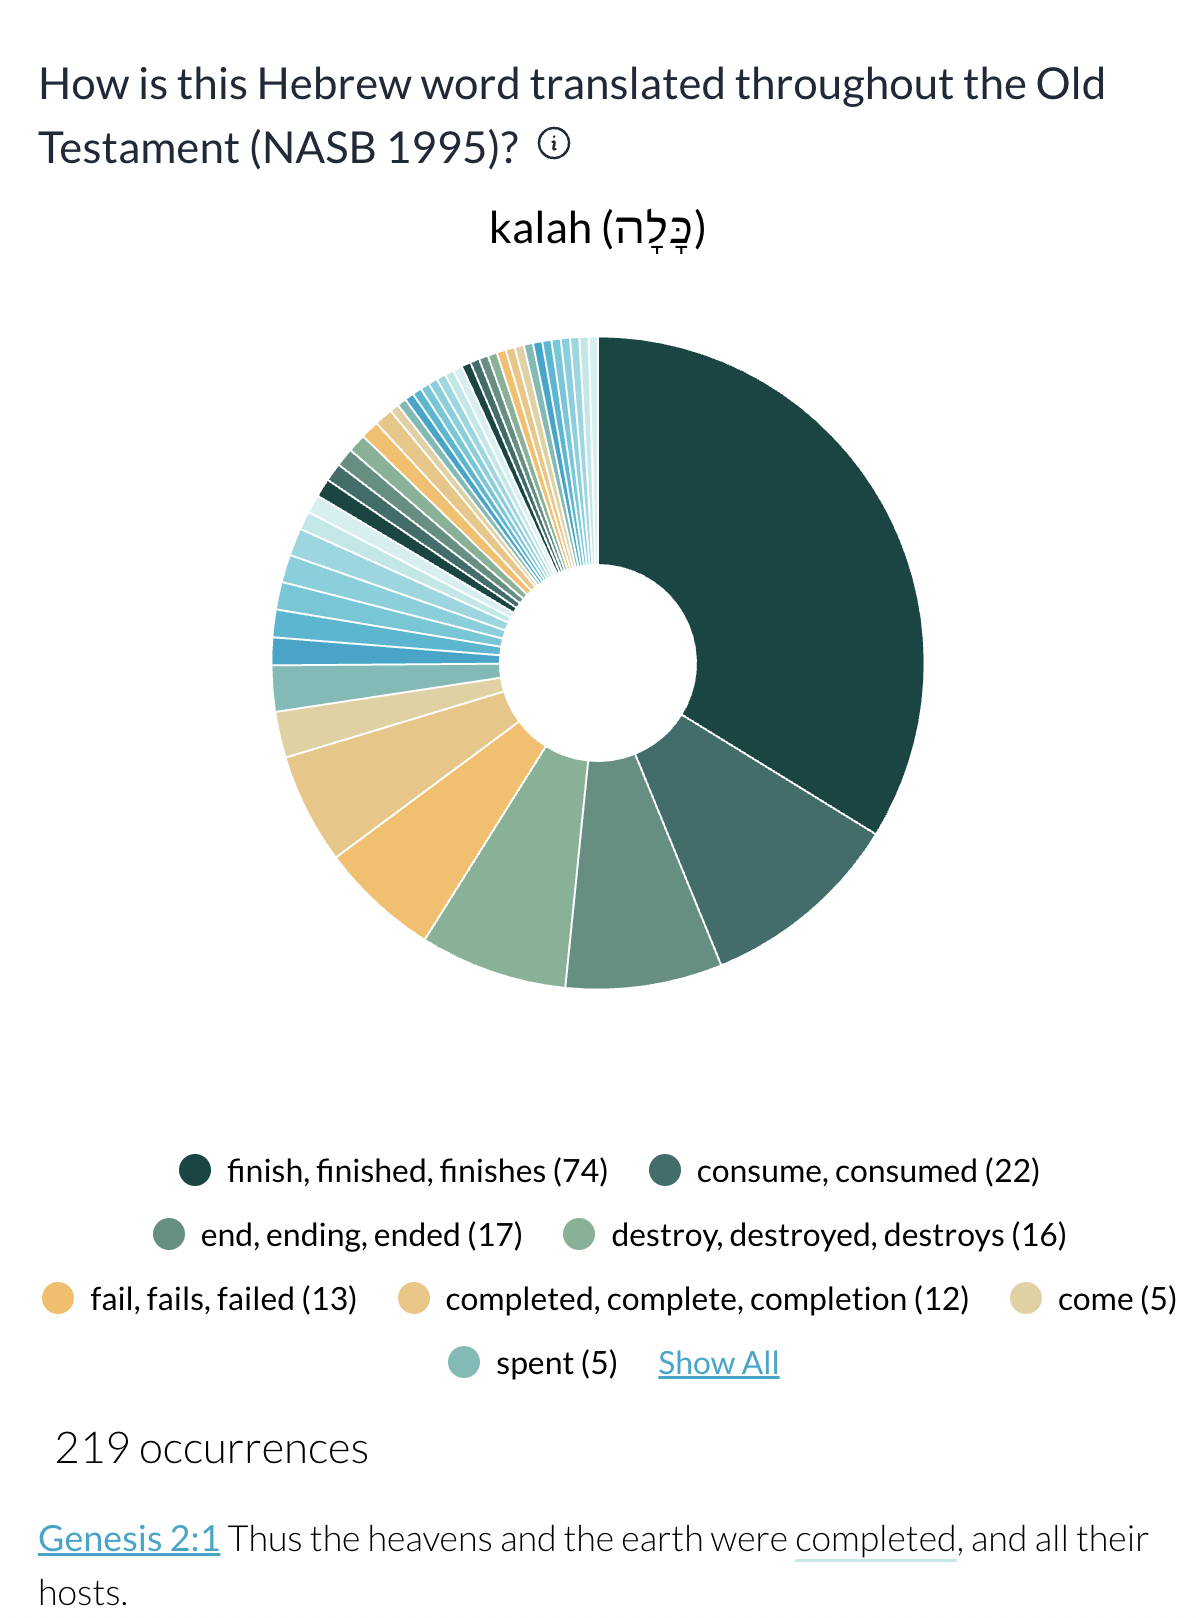
\includegraphics[width=0.75\columnwidth]{figures/word-donut.png}
  \caption{The Word Donut visualization for the Hebrew word \textit{kalah}, showing how it is rendered across 221 Old Testament occurrences. Segments represent distinct English renderings (e.g., ``finish'' 74$\times$, ``consume'' 24$\times$), enabling readers to explore semantic range without knowledge of the original language.}
  \label{fig:word-donut}
\end{figure}

\paragraph{User experience and data flow.}
The application provides dark mode, adjustable font sizes, mobile-responsive layout, deep linking via URL parameters (e.g., \texttt{/read?v=Matthew.1.1}), and an in-app feedback system; the UI underwent four rounds of dedicated usability testing, including tests focused specifically on the drawer navigation and the Word Donut. Pre-generated BHTs from the BibleGoAI pipeline are loaded into a PostgreSQL database and served by the Next.js application through server-side API routes; Bible text with Strong's tags is served from static JSON files, while Strong's concordance entries are queried from the database.
